%------------------------------------------------------------------------------------
%	CHAPTER 1
%------------------------------------------------------------------------------------
\chapterimage{headMontagem.png}
\chapter{Entendimento Geral}

\begin{remark}
"Um bom programador não se define pelas ferramentas que usa, mas pelo que aprende ao dominá-las — como o Pascal ensina." (\textit{Alan Perlis}, primeiro vencedor do prêmio Turing.) 
\end{remark}

\section{Do que trata esse livro?}\index{Entendimento Geral}
\textbf{Pascal} foi criada em 1970 pelo cientista da computação suíço \textbf{Niklaus Wirth}. Seu objetivo principal foi desenvolver uma linguagem que fosse eficiente, fácil de aprender e que promovesse boas práticas de programação, como por exemplo, o ensino da Lógica de Programação. Inspirada por linguagens anteriores como \textbf{ALGOL}, \textbf{Pascal} foi projetada para ensinar conceitos fundamentais de programação estruturada e desenvolvimento de software, sendo amplamente adotada em ambientes acadêmicos durante as décadas de 1970 e 1980.

O nome da linguagem é uma homenagem ao matemático e filósofo francês \textbf{Blaise Pascal}, conhecido por suas contribuições à matemática e pela invenção de uma das primeiras calculadoras mecânicas, como a \textit{Pascalina}\footnote{A Pascalina foi uma das primeiras calculadoras mecânicas da história, criada pelo matemático, físico e filósofo francês \textbf{Blaise Pascal} em 1642, quando ele tinha apenas 19 anos. Foi projetada para ajudar seu pai, \textbf{Étienne Pascal}, que trabalhava como coletor de impostos e precisava realizar muitos cálculos repetitivos. A invenção marcou um marco significativo no desenvolvimento das máquinas de cálculo.}. A linguagem Pascal trouxe inovações importantes, como a ênfase em estruturas de controle claras (condicionais e laços) e na organização modular de programas, o que ajudou os desenvolvedores a criar código legível e fácil de manter.

Embora inicialmente projetada para ensinar, a linguagem logo encontrou aplicações práticas na indústria. Versões como \textbf{Turbo Pascal}, lançada pela \textbf{Borland} na década de 1980, tornaram-se extremamente populares devido à sua rapidez, facilidade de uso e baixo custo. \textbf{Turbo Pascal} oferecia um ambiente de desenvolvimento integrado (IDE) que permitia aos programadores escrever, compilar e executar programas de forma eficiente, algo revolucionário para a época.

Ao longo do tempo, \textbf{Pascal} evoluiu e deu origem a variantes como \textbf{Object Pascal}, que introduziu conceitos de programação orientada a objetos e serviu de base para o desenvolvimento de ferramentas como o \textbf{Delphi}, um ambiente robusto para criar aplicações gráficas para o sistema \textbf{Windows} (na época seu único concorrente era o Visual Basic da própria \textbf{Microsoft}).

Embora Pascal tenha perdido popularidade com o surgimento de linguagens mais modernas derivadas do \textbf{C}, sua influência persiste. Muitos programadores veteranos aprenderam conceitos fundamentais de computação usando o \textbf{Pascal}, e sua ênfase em clareza e estrutura continua sendo uma lição valiosa para a programação até hoje.

\section{Quais são as vantagens de se aprender Pascal atualmente?}\index{Entendimento Geral}
Aprender a linguagem Pascal hoje pode oferecer algumas vantagens, dependendo do contexto e do objetivo de aprendizado. Aqui estão algumas delas:
\begin{itemize}
	\item \textbf{Fundamentos de programação}: é uma linguagem muito boa para aprender os conceitos básicos de programação, como variáveis, estruturas de controle, funções e tipos de dados. Sua sintaxe simples e clara ajuda a focar no raciocínio lógico sem sobrecarregar o aluno com complexidade.
	\item \textbf{Educação}: universidades e escolas a usam como linguagem introdutória em cursos de ciência da computação no passado. Embora outras linguagens tenham substituído em muitos lugares, a base sólida que Pascal oferece ainda é valiosa em cursos que ensinam os fundamentos da programação.
	\item \textbf{Histórico e legado}: o conhecimento pode ser útil caso seja necessário trabalhar em projetos legados ou sistemas que ainda utilizam essa linguagem. Alguns softwares mais antigos, especialmente em áreas como automação industrial e sistemas embarcados, são escritos em Pascal e exigem conhecimento nesta (seja para manutenção ou mesmo migração).
	\item \textbf{Clareza e estrutura}: \textbf{Pascal} foi projetada para ser fácil de entender e ensinar. Sua sintaxe é bastante rígida, o que pode ajudar a evitar maus hábitos na programação.
	\item \textbf{Portabilidade}: compiladores modernos para Pascal (como \textbf{Free Pascal}) que permitem rodar o código em diferentes plataformas. Isso pode ser interessante para quem deseja experimentar linguagens de baixo nível ou desenvolver software que precise ser altamente eficiente.
	\item \textbf{Desenvolvimento de algoritmos}: sendo uma linguagem estruturada, é muito boa para o desenvolvimento e análise de algoritmos, sem a complexidade de recursos modernos visto em outras linguagens.
\end{itemize}
Essas vantagens tornam o COBOL uma escolha interessante para quem deseja trabalhar em áreas que envolvem sistemas legados e infraestrutura crítica, permite abrir portas para um conjunto especializado de habilidades que ainda tem grande valor no mercado de trabalho.

\section{Montagem do Ambiente}\index{Entendimento Geral}
Podemos montar nosso ambiente de desenvolvimento sobre diversos sistemas operacionais, oferecendo flexibilidade na escolha da plataforma ideal para o projeto. Neste livro, é utilizado o Ubuntu 24.10, uma das distribuições Linux mais populares e acessíveis, conhecida por sua estabilidade, segurança e suporte a uma vasta gama de ferramentas de desenvolvimento.

O uso de software livre é uma das principais vantagens deste ambiente, pois todos os programas e bibliotecas necessárias para o desenvolvimento estarão disponíveis gratuitamente, sem custos adicionais. Isso inclui editores de código, ferramentas de automação e depuração, que são perfeitamente adequados para projetos profissionais. Além disso, o hardware necessário é simples: um computador (que provavelmente já possui), sem a necessidade de investimentos adicionais em equipamentos especializados. Com isso, podemos configurar um ambiente de desenvolvimento poderoso e eficiente, aproveitando ao máximo os recursos do Ubuntu e dos softwares livres, sem comprometer o orçamento.

Iremos utilizar o \textbf{Free Pascal}, assim na tela de terminal usamos o seguinte comando: \\
\codigo{\$ sudo apt install fpc}

Necessitamos de um editor de códigos, recomendo o Visual Studio Code, não apenas pela leveza pois, dentre todos os editores é o que melhor se adapta a linguagem Pascal através dos plugins. \\
\codigo{\$ snap install code}

Criamos uma pasta para manter nossos códigos arrumados: \\
\codigo{\$ mkdir pascalProjects}

Entramos nessa pasta: \\
\codigo{\$ cd pascalProjects}

E no editor: \\
\codigo{\$ code .}

Na seção \textbf{Extensões}, instalamos o seguinte plugin:
\begin{itemize}
	\item FreePascal Toolkit - Fornecedor: coolchyni
\end{itemize}

E agora estamos prontos para criarmos e executarmos nosso primeiro programa em máquinas atuais na linguagem Pascal.

\section{Mais sobre a Pascalina}\index{Entendimento Geral}
As pessoas confundem a \textbf{Pascalina} (calculadora criada por \textbf{Blaise Pascal}) com a Máquina Diferencial (1822) de \textbf{Charles Babbage}, que era também um dispositivo mecânico para calcular e imprimir tabelas matemáticas, como as de logaritmos.

\begin{figure}[H]
	\centering
	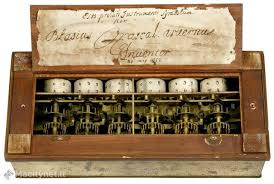
\includegraphics[width=0.5\textwidth]{cap01/pascalina.jpeg}
	\caption{Pascalina}
\end{figure}

A \textbf{Pascalina} era uma máquina baseada em engrenagens que podia realizar operações básicas de adição e subtração. Seu mecanismo utilizava rodas dentadas numeradas de 0 a 9, conectadas de forma que, ao girar uma roda, os números fossem ajustados automaticamente. O sistema implementava a ideia de "transbordo" (ou carry), em que, ao ultrapassar o valor 9, uma roda fazia a próxima avançar, semelhante ao funcionamento dos odômetros. 

Embora a Pascalina fosse uma tecnologia revolucionária para a época, ela não teve ampla adoção devido ao seu alto custo de fabricação e à complexidade de operação. Ainda assim, a máquina é considerada um marco na história da computação, pois foi uma das primeiras tentativas de automatizar cálculos, reduzindo o esforço humano e os erros associados ao trabalho manual. Atualmente está preservada em museus e representada em reproduções, e continua sendo um símbolo da engenhosidade humana e um precursor das modernas calculadoras e computadores.

Se deseja conhecer mais sobre esse fantástico projeto, assista o vídeo do Canal "What Will Makes" \url{https://www.youtube.com/watch?v=E0pJST5mL3A&t=2s}, onde um jovem engenheiro mostra passo a passo da execução de um projeto similar.

\clearpage